\begin{lemma}
    Пусть простая гладкая поверхность $S = \bigcup\limits_{i = 1}^N S_i$~---~объединение простых гладких поверхностей, пересекающихся только по краям, $f \in C(S, \R)$. Тогда \[\iint\limits_S fds = \sum\limits_{i = 1}^N \iint\limits_{S_i} fds\]
\end{lemma}
\begin{proof}
    Очевидно следует из определения и аддитивности интеграла.
\end{proof}
\begin{definition}
    Пусть $S = \overline{r}(\overline{G})$~---~кусочно-гладкая поверхность. Пусть $f \in C(S, \R)$. Тогда если $S = \bigcup\limits_{i = 1}^N S_i$, то по определению \[\iint\limits_S fds = \sum\limits_{i = 1}^N \iint\limits_{S_i} fds\]
\end{definition}
\begin{fact}[Доказательство оставлено в качестве упражнения]
    Определение корректно, и доказательство аналогично доказательству корректности интеграла Лебега от простых функций.
\end{fact}
\begin{theorem}
    ПИПР не зависит от параметризации поверхности.
\end{theorem}
\begin{proof}
    Достаточно рассмотреть случай простой гладкой поверхности. Пусть $S = \overline{r}(\overline{G}) = \overline{r} \circ w(\overline{\Omega})$ где $\overline{\Omega} \xleftrightarrow{w} \overline{G}$ и $J_w \neq 0$ в любой точке $\overline{\Omega}$. Пусть \begin{equation*}
        w(\alpha, \beta) = \begin{pmatrix}
            u(\alpha, \beta) \\ v(\alpha, \beta)
        \end{pmatrix}
    \end{equation*}
    Пусть $f \in C(S, \R)$. Тогда \[\iint\limits_S fds = \iint\limits_{\overline{G}} f(\overline{r}(u, v))|[\overline{r}'_u \times \overline{r}'_v]|dudv = \iint\limits_{\overline{\Omega}} f(\overline{r}\circ w(\alpha, \beta))|[\overline{r}'_u(\alpha, \beta) \times \overline{r}'_v(\alpha, \beta)]||J_w|d\alpha d\beta = \]\[ = \iint\limits_{\overline{\Omega}} f(R(\alpha, \beta))|[\overline{R}'_\alpha(\alpha, \beta) \times \overline{R}'_\beta(\alpha, \beta)]|d\alpha d\beta\] 
    Где $\overline{R} = \overline{r} \circ w$.
\end{proof}
\begin{lemma}
    Пусть \[S = \{\overline{r}(x, y) = \begin{pmatrix}
        x \\ y \\ z(x, y)
    \end{pmatrix} \mid (x, y) \in \overline{G} \}\]
    Для некоторой $z \in C^1(\overline{G}, \R)$. Тогда \[\iint\limits_S f(x, y, z)ds = \iint\limits_G f(x, y, z(x, y))\sqrt{1 + (z'_x)^2 + (z'_y)^2}dxdy\]
\end{lemma}
\begin{proof}
    Поскольку \[
    \overline{r}'_x = \begin{pmatrix}
        1 \\ 0 \\ z'_x
    \end{pmatrix}, \quad \overline{r}'_y = \begin{pmatrix}
        0 \\ 1 \\ z'_y
    \end{pmatrix}
    \]
    Тогда $|[\overline{r}'_x \times \overline{r}'_y]| = \sqrt{|\overline{r}'_x|^2|\overline{r}'_y|^2 - (\overline{r}'_x\cdot \overline{r}'_y)^2} = \sqrt{1 + (z'_x)^2 + (z'_y)^2}$
\end{proof}

\subsection{Поверхностный интеграл II рода}
Физический смысл --- это поток векторного поля через поверхность в направлении, задаваемой нормалью
\begin{definition}
    Пусть $S = \overline{r}(\overline{G})$~---~кусочно-гладкая поверхность, ориентированная полем единичных нормалей $\overline{n}$. Пусть $\overline{F} \in C(S, \R^3)$ и \[
    \overline{F} = 
    \begin{pmatrix}
        P \\ Q \\ R
    \end{pmatrix}
    \]
    Тогда определим интеграл второго рода как \[
    \iint\limits_S (\overline{F}, \overline{ds}) = \iint\limits_S Pdydz + Qdzdx + Rdxdy := \iint\limits_S (\overline{F}, \overline{n})ds
    \]
\end{definition}
\begin{lemma}
    Не зависит от параметризации поверхности (при сохранении ориентации поверхности те $J_F > 0$)
\end{lemma}
\begin{proof}   
    Поскольку ПИПР не зависит от параметризации, и поле нормалей тоже не зависит от параметризации то интеграл не изменится.
\end{proof}
\begin{lemma}
    Пусть $S = \overline{r}(\overline{G})$~---~простая ориентированная гладкая поверхность. Пусть $\overline{F} \in C(S, \R^3), \overline{F} = (P \ Q \ R)^T$. Тогда \[\iint\limits_S (\overline{F}, \overline{ds}) = \pm \iint\limits_G \begin{vmatrix}
        P & Q & R \\ x'_u & y'_u & z'_u \\ x'_v & y'_v & z'_v
    \end{vmatrix} dudv
    \]
    Определяется $\pm$ по ориентации поверхности. Пусть $\overline{r}_0 = \overline{r}(u_0, v_0) \in S$. Если $\overline{n}(\overline{r}_0)$ и $[\overline{r}'_u(u_0, v_0) \times \overline{r}'_v(u_0, v_0)]$ сонаправлены, то <<+>>, иначе -- <<->>.
\end{lemma}
\begin{proof}
    Для производной простой гладкой поверхности поле нормалей выглядит как \[\overline{n}(\overline{r}) = \pm\dfrac{\overline{r}'_u \times \overline{r}'_v}{|\overline{r}'_u \times \overline{r}'_v|}\]
    Знак выбирается в зависимости от изначальной ориентации поверхности. Тогда \[
    \iint\limits_S (\overline{F}, \overline{ds}) = \iint\limits_{S}(\overline{F}, \overline{n})ds = \iint\limits_G (\overline{F}(\overline{r}(u, v)), \overline{n}(\overline{r}(u, v)))|\overline{r}'_u \times \overline{r}'_v|dudv = \]\[ =  \pm\iint\limits_G (\overline{F}(\overline{r}(u, v)), \overline{r}'_u(u, v) \times \overline{r}'_v(u, v))dudv = \pm \iint\limits_G \begin{vmatrix}
        P & Q & R \\ x'_u & y'_u & z'_u \\ x'_v & y'_v & z'_v
    \end{vmatrix} dudv
    \]
\end{proof}
\hypertarget{graph_gaus}{}
\begin{theorem}
    Пусть $G \subset \R^2_{xy}$~---~область с границей, являющейся простым гладким кусочно гладким контуром и $z \in C^1(\overline{G})$ и $S = \graph z$. Пусть $S^+$~---~поверхность $S$, ориентированная полем нормалей $\overline{n} = (n_x \  n_y \  n_z)^T$ таким, что $n_z \geq 0$. Тогда \[
    \iint\limits_{S^+} f(x, y, z)dxdy = \iint\limits_G f(x, y, z(x, y))dxdy
    \]
\end{theorem}
\begin{proof}
    Пусть \begin{equation*}
        \overline{r}(x, y) = \begin{pmatrix}
            x \\ y \\ z(x, y)
        \end{pmatrix} \Rightarrow \overline{r}'_x = \begin{pmatrix}
            1 \\ 0 \\ z'_x
        \end{pmatrix}, \quad \overline{r}'_y = \begin{pmatrix}
            0 \\ 1 \\ z'_y
        \end{pmatrix}
    \end{equation*}
    Тогда используя предыдущую лемму и то, что $\overline{F} = (0 \ 0 \ f)^T$, то мы получаем, что \[
    \iint\limits_S fdxdy = \iint\limits_G \begin{vmatrix}
        0 & 0 & f \\ 1 & 0 & z'_x \\ 0 & 1 & z'_y
    \end{vmatrix}dxdy =  \iint\limits_G f(x, y, z(x, y))dxdy
    \]
\end{proof}

\subsection{Формула Остроградского-Гаусса}
\begin{definition}
    Будем называть наблой формальный дифференциальный оператор $\nabla$: \[
        \nabla = \begin{pmatrix}
            \dfrac{\partial}{\partial x} \\ \dfrac{\partial}{\partial y} \\ \dfrac{\partial}{\partial z}
        \end{pmatrix}
    \]
    Он действует следующим образом: \[
        \nabla(\sum\limits_i \alpha_i p_i) = \sum\limits_i \alpha_i \nabla p_i
    \]
    (Если $\alpha_i$~---~константы) \\
    Набла удовлетворяет правилу Лейбница: \[
        \nabla(pq) = \nabla(\overset{\downarrow}{p}, q) + \nabla(p, \overset{\downarrow}{q}) = (\nabla p, q) + (p, \nabla q)
    \]
\end{definition}
\begin{definition}
    Определим операцию взятия градиента как \[\grad a = \nabla a = \begin{pmatrix}
\frac{\partial a}{\partial x} \\
\frac{\partial a}{\partial y} \\
\frac{\partial a}{\partial z}
\end{pmatrix}.
\]
\end{definition}
\begin{definition}
    Определим дивергенцию векторного поля как \[\div \overline{F} = \nabla \cdot \overline{F} = \frac{\partial F_x}{\partial x} + \frac{\partial F_y}{\partial y} + \frac{\partial F_z}{\partial z}.
\]
\end{definition}
\begin{definition}
    Определим операцию взятия ротора как \[\rot \overline{F} = \nabla \times \overline{F} = \begin{pmatrix}
\frac{\partial F_z}{\partial y} - \frac{\partial F_y}{\partial z} \\
\frac{\partial F_x}{\partial z} - \frac{\partial F_z}{\partial x} \\
\frac{\partial F_y}{\partial x} - \frac{\partial F_x}{\partial y}
\end{pmatrix}.
\]
\end{definition}
\begin{note}(от редактора)
\begin{itemize}
    \item Геометрический смысл дивергенции заключается в том, что это предел отношения потока векторного поля через замкнутую поверхность, окружающую данную точку, к объёму, ограниченному этой поверхностью, когда она стягивается к точке. Вспомните теорему Гаусса, если взять заряд, то поток будет равен $4 \pi q_{in}$.
    \item Геометрический смысл ротора заключается в том, что это циркуляция по малому контуру, то, насколько в конкретной точке поток поворачивается. Представьте закрепленный шарик в воде, за счет вязкости этот шарик будет вращаться в каком-то направлении, а угловая скорость вращения это удвоенное значение ротора
\end{itemize}



\end{note}
\begin{definition}
    Область $G$ называют сильно элементарной область в $\R^3_{xyz}$, если она элементарна относительно каждой из осей.
\end{definition}
\begin{definition}
    Будем говорить, что обалсть $G$ элементарна относительно $Oz$, т.е. $\exists E \in \R^2_{xy}$ такая, что $G = \{(x, y, z) \mid (x, y) \in E, z \in (\phi(x, y), \psi(x, y))\}$ где $\phi(x, y)$ и $\psi(x, y)$~---~гладкие в $\overline{E}$
\end{definition}

\begin{theorem}
    Пусть $G$~---~ сильно элементарная область в $\R^3_{xyz}$. Пусть $\partial G$~---~кусочно-гладкая поверхность, ориентированная полем внешних нормалей. Пусть $\overline{F} \in C^1(\overline{G}, \R^3)$. Тогда \[\iiint\limits_{G} \div \overline{F} dxdydz = \iint\limits_{\partial G^+} (\overline{F}, \overline{ds})\]
\end{theorem}
\begin{proof}
    Пусть \[\overline{F} = \begin{pmatrix}
        P \\ Q \\ R
    \end{pmatrix}\]
    Тогда, необходимо доказать, что \[\iiint\limits_G \div \overline{F} dxdydz = \iiint\limits_G P'_x + Q'_y + R'_z dxdydz = \iint\limits_{\partial G^+} Pdydz + Qdxdz + Rdxdy\]
    В силу линейности интеграла мы можем доказать только для одной из компонент $\overline{F}$. Пусть это будет, без ограничения общности, \[\overline{F}_3 = \begin{pmatrix}
        0 \\ 0 \\ R
    \end{pmatrix}\]
    Тогда, необходимо доказать \[\iiint\limits_G R'_z dxdydz = \iint\limits_{\partial G^+} Rdxdy\]
    Поскольку $G$~---~элементарно относительно $Oz$, то существует $E \subset \R^2_{xy}$ и $\psi, \phi \in C^1(\overline{E}, \R)$ т.ч. $\phi < \psi$. Тогда \[G = \{(x, y, z) \mid (x, y) \in E, \phi(x, y) < z < \psi(x, y)\}\]

    \noindent 
    \begin{minipage}{0.5\textwidth}
    Введём следующие обозначения: \[S_1 = \{(x, y, \psi(x, y)) \mid (x, y) \in \overline{E}\}\]
    \[S_2 = \{(x, y, \phi(x, y)) \mid (x, y) \in \overline{E}\}\]
    \[S_3 = \{(x, y, z) \mid (x, y) \in \partial E, \phi \leq z \leq \psi\}\]
    Поскольку поле внешних нормалей к $S_3$ параллельно плоскости плоскости $Oxy$, а следовательно его $z$-компонента $n_z = 0$. Тогда \[\iint\limits_{S_3} Rdxdy = \iint\limits_{S_3} R \cdot n_z ds = 0\]
    \end{minipage}
    \begin{minipage}{0.55\textwidth}
    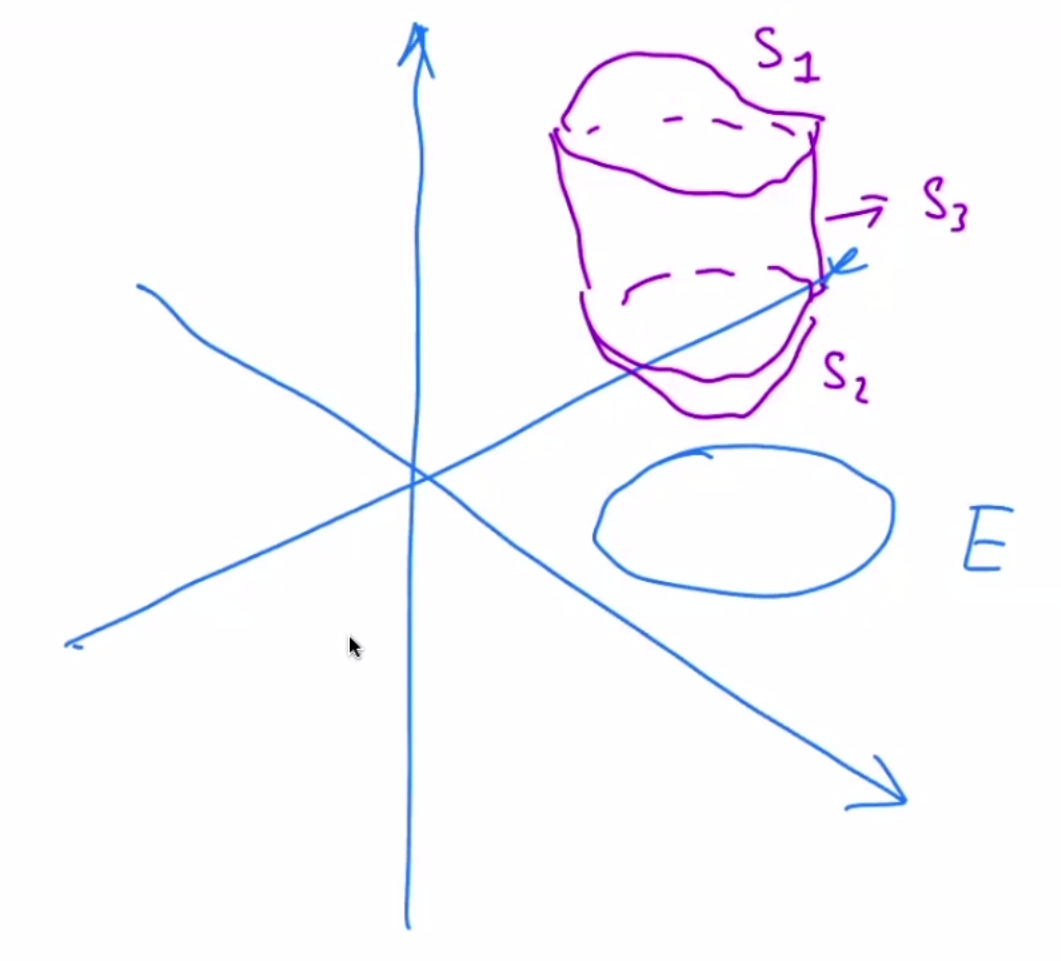
\includegraphics[width=\textwidth]{images/minigaus.png}
    \end{minipage}
    В тоже время, \hyperlink{graph_gaus}{по теореме о вычислении поверхностного интеграла в случае графика:} \[\iint\limits_{S_1} Rdxdy = \iint\limits_E R(x, y, \psi(x, y))dxdy\] \[\iint\limits_{S_2} Rdxdxy = -\iint\limits_{E} R(x, y, \phi(x, y))dxdy\]
    Но, тогда \[\iint\limits_{\partial G^+} Rdxdy = \iint\limits_{S_1}Rdxdy + \iint\limits_{S_2}Rdxdy + \iint\limits_{S_3}Rdxdy = \iint\limits_E R(x, y, \psi(x, y)) - R(x, y, \phi(x, y))dxdy = \]
    Тогда по формуле Ньютона-Лейбница (так как поле непрерывно дифференцируемо в замыкании), а в конце по принципу Кавальери: \[ = \iint\limits_{E} \biggr(\int\limits_{\phi(x, y)}^{\psi(x, y)} R'_z(x, y, t)dt\biggr) dxdy = \iiint\limits_G R'_zdxdydz\]
    Теорема доказана (для остальных компонент результат получается аналогично)
\end{proof}
\begin{theorem}[Остроградский, Гаусс]
    Пусть есть область $G$, т.ч. $G = \bigcup\limits_{i = 1}^N \cup E$ где $G_i$~---~элементарные области, а $E = \bigcup\limits_{j = 1}^N S_j$, где $S_j$~---~кусочно-гладкие поверхности, лежащие на границах областей $G_i$. Пусть $\partial G^+$~---~кусочно-гладкая поверхность, ориентированная полем внешних нормалей. И пусть задано $\overline{F} \in C^1(G, \R^3)$. Тогда \[\iiint\limits_{G} \div \overline{F} dxdydz = \iint\limits_{\partial G^+} (\overline{F}, \overline{ds})\]
\end{theorem}
\begin{proof}
    Для каждой из элементарных областей справедливо утверждение предыдущей теоремы: \[\iiint\limits_{G_i} \div \overline{F} dxdydz = \iint\limits_{\partial G_i^+} (\overline{F}, \overline{ds})\]
    Очевидно, что \[\iiint\limits_{G} \div \overline{F} dxdydz = \sum\limits_{i = 1}^N \iiint\limits_{G_i}\div \overline{F} dxdydz\]
    Поскольку $\LL^3$ для кусочно-гладкой поверхности равна $0$. С другой стороны, пусть $S_{il}$~---~общая часть границы $G_i$ и $G_l$. Заметим, что если $S^+_{il}$~---~внешне-ориентирована по отношению к $G_i$, то она же будет внутренне ориентирована по отношению к $G_l$. А значит, в сумме интегралов по всем $\partial G^+_i$ они все взаимно уничтожатся, и тогда справедливо \[\sum\limits_{i = 1}^N (\overline{F}, \overline{ds}) = \iint\limits_{\partial G^+} (\overline{F}, \overline{ds})\]
    Теорема доказана.
\end{proof}